\documentclass[11pt]{article}

\usepackage[margin=1in]{geometry}
\usepackage{amsmath,amssymb}
\usepackage{booktabs}
\usepackage{graphicx}
\usepackage[dvipsnames]{xcolor}
\usepackage[colorlinks=true,linkcolor=NavyBlue,urlcolor=NavyBlue]{hyperref}
\usepackage{caption}
\usepackage{fancyhdr}

\captionsetup{font=small,labelfont=bf}
\pagestyle{fancy}
\fancyhf{}
\fancyhead[L]{\small STAT 638 --- what the new exploratory analysis shows}
\fancyhead[R]{\small\thepage}
\renewcommand{\headrulewidth}{0.4pt}

\newcommand{\kwh}{\,\mathrm{kWh}}

\title{\vspace{-1.2cm}\textbf{What the new exploratory analysis shows}\\[4pt]
\large Household electricity demand, before the Bayesian model}
\author{Project 17}
\date{\today}

\begin{document}
\maketitle
\thispagestyle{fancy}

\begin{abstract}
\noindent
The first pass at the data checked the response scale and the residual
autocorrelation. This note is the deeper pass: where the day-to-day variance
sits, why August looks so low, which circuits carry the winter peak, and why
the weekend effect is not one number. The fits below are ordinary least
squares. Intervals are descriptive Newey--West intervals, not the posteriors
in the main report. The same material is written into the technical report;
this PDF is the reading version.
\end{abstract}

\section{What was added}

The new script, \texttt{src/01d\_indepth\_eda.py}, stays on the daily series
already built from the minute data: $1{,}417$ days with at least 95\% of their
minutes observed, from 17 December 2006 to 25 November 2010. It adds five
things the earlier checks did not do.

\begin{enumerate}
\item A sequential variance split on the kWh scale: trend, then each annual
harmonic, then day of week, with month indicators as a ceiling.
\item The shape of the year, year by year, against one harmonic and against
two, together with the within-month spread.
\item A split of each day into the three sub-meters and the unmetered
remainder, by month and for the August 2008 vacancy.
\item The weekly pattern after month effects, including a separate
weekend-minus-weekday contrast in each season, and the average power through
the hours of a winter day and a summer day.
\item A trend slope under several cuts of the sample, and a check that French
public holidays are not a missing mean term.
\end{enumerate}

The dependence checks in this pass are on the kWh scale, which is the scale
the held-out forecasts later prefer.

\section{Six findings}

\subsection{The calendar explains under half of a day, and almost all of that is one wave}

\begin{center}
\small
\begin{tabular}{@{}lrrr@{}}
\toprule
Specification & $R^2$ & Increment & Residual SD \\
\midrule
Intercept only & 0.000 & 0.000 & 10.00 \\
Linear trend & 0.011 & 0.011 & 9.94 \\
Add first harmonic & 0.375 & 0.364 & 7.90 \\
Add second harmonic & 0.400 & 0.024 & 7.75 \\
Add day of week & 0.452 & 0.052 & 7.40 \\
Add third harmonic & 0.467 & 0.015 & 7.30 \\
Add fourth harmonic & 0.478 & 0.011 & 7.22 \\
\addlinespace
Trend + month + day of week & 0.470 & --- & 7.28 \\
\bottomrule
\end{tabular}

\end{center}

\noindent
Each row adds the named terms to the rows above it. The last row replaces the
harmonics with a separate level for each month; it is a ceiling, not a further
step.

A linear trend adds $R^2 = 0.011$. The first harmonic adds $0.364$, which is
four fifths of the $R^2 = 0.452$ reached by trend, two harmonics, and day of
week together. The second harmonic adds $0.024$. Day of week adds $0.052$.
The residual standard deviation is then $7.40\kwh$, against $10.00\kwh$ with
no structure at all. A bit over half of the variation from day to day is still
left over. That is why the predictive intervals in the main analysis are wide:
the calendar is real, and a typical day still sits several kWh off it.

The third and fourth harmonics add $0.015$ and $0.011$. Letting every month
have its own level, on top of the trend and day of week, reaches
$R^2 = 0.470$, only $0.018$ above two harmonics. Two harmonics already carry
the season. What they miss is a small lack of fit.

A single weekend indicator, after month effects, adds $0.046$. Giving the
other weekdays their own levels adds only $0.007$ more. The weekend is the
weekly variance. Monday and Thursday are still low, by about $2$--$3\kwh$,
but that pattern is a small slice of $R^2$.

\subsection{August's mean of 13.7 kWh is a mixture}

\begin{figure}[htbp]
\centering
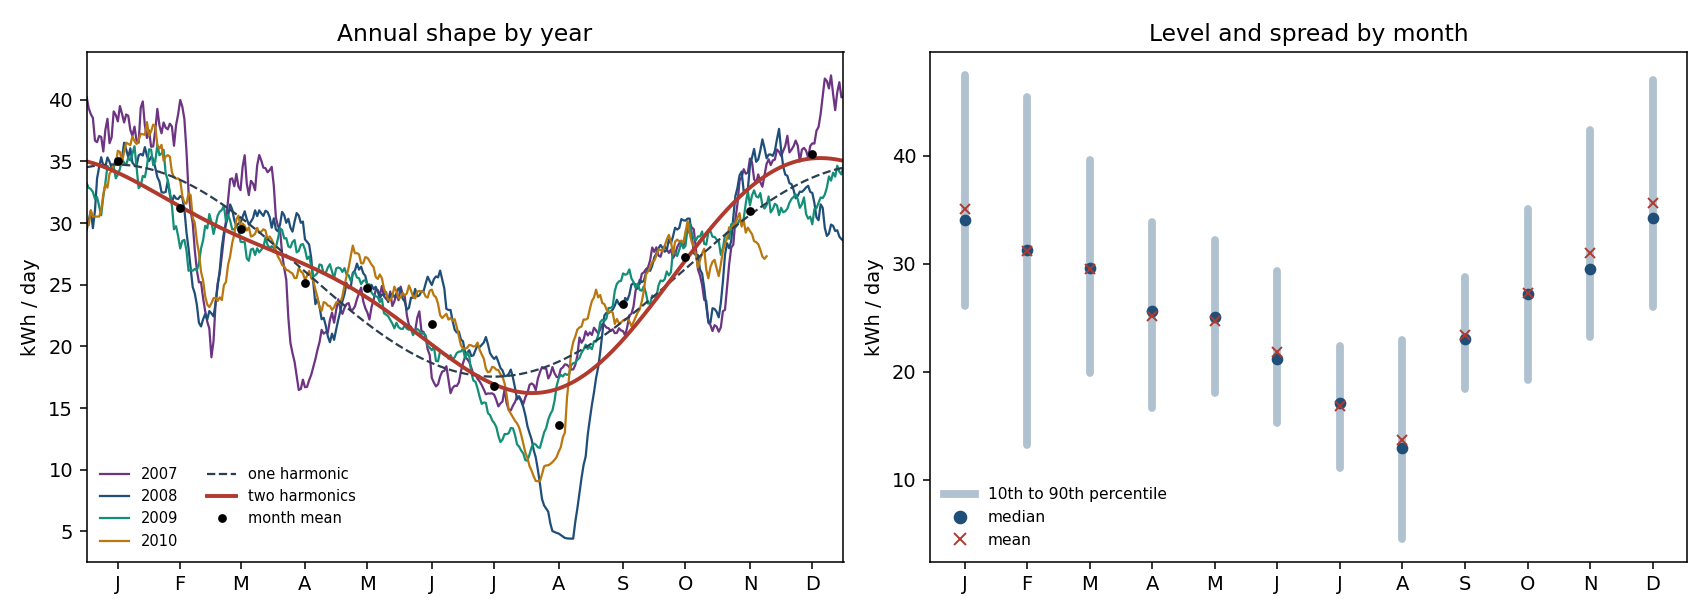
\includegraphics[width=\textwidth]{figures/01d_seasonal.png}
\caption{Left: a 15-day moving average in each year, the month means, and the
seasonal curve with one harmonic and with two. The 2008 collapse in August is
the vacant stretch. Right: within each month, the 10th to the 90th percentile,
the median, and the mean.}
\end{figure}

With one harmonic the fitted curve peaks on 14 January at $34.8\kwh$ and
troughs on 16 July at $17.6\kwh$: a range of $17.2\kwh$, amplitude $8.6\kwh$.
Two harmonics move the crest to 20 December and the trough to 3 August, and
stretch the range to $19.1\kwh$. The second harmonic's own amplitude is
$2.2\kwh$. The gain is the shape: a later, deeper summer floor, and a crest
that sits in late December rather than a symmetric half-year away from
mid-July.

The same shape repeats. Correlations of the twelve monthly means between years
are $0.89$ to $0.93$, except 2007 against 2008 at $0.77$, and that exception
is August 2008.

Of 117 retained August days, 47 fall in a run of at least five days under
$12\kwh$. The other 70 average $18.30\kwh$ (median $18.18$). July averages
$16.81\kwh$. An occupied summer is about $17$--$18\kwh$ a day. The published
August mean of $13.67\kwh$, and the August median of $12.93$, sit that low
because the vacancies are about two fifths of the August sample, enough to
reach the middle. The 10th percentile is $4.54\kwh$ and the 90th is $22.91$.
The two-harmonic trough, $16.2\kwh$, falls between the raw August mean and the
occupied-August mean. The notch to about $5\kwh$ on the 2008 curve is an empty
house, not a second climate.

From 6 to 30 August 2008 the house averaged $4.76\kwh$ a day, which is
$0.20\,\mathrm{kW}$ running continuously. The kitchen contribution that
fortnight is zero. July 2008 averaged $19.07\kwh$, and August 2007, the August
with no long vacancy, averaged $18.33\kwh$. Those two match.

December needs a smaller version of the same caution. The fifteen days of
December 2006 average $45.1\kwh$; later Decembers average $34.1$. The record
opens on its highest fortnight. The maximum, $79.6\kwh$ on 23 December 2006,
is in it.

Public holidays are not a missing piece of the mean. Across 43 retained
holiday dates, the residual after month and day-of-week means is
$+0.4\kwh$. Christmas is high in two years and low in 2008. The last week of
December runs $2.2\kwh$ above the rest of December, with a standard error of
$2.5$.

\subsection{The winter peak is heating and hot water}

\begin{center}
\small
\begin{tabular}{@{}lrrrr@{}}
\toprule
End use & Mean & Share & Dec$-$Aug & Share of gap \\
\midrule
Unmetered & 13.41 & 51.2\% & +14.20 & 64.6\% \\
Water heater and air conditioner & 9.30 & 35.5\% & +5.67 & 25.8\% \\
Laundry & 1.87 & 7.1\% & +0.94 & 4.3\% \\
Kitchen & 1.61 & 6.2\% & +1.17 & 5.3\% \\
Total & 26.19 & 100\% & +21.97 & 100\% \\
\bottomrule
\end{tabular}

\end{center}

\begin{figure}[htbp]
\centering
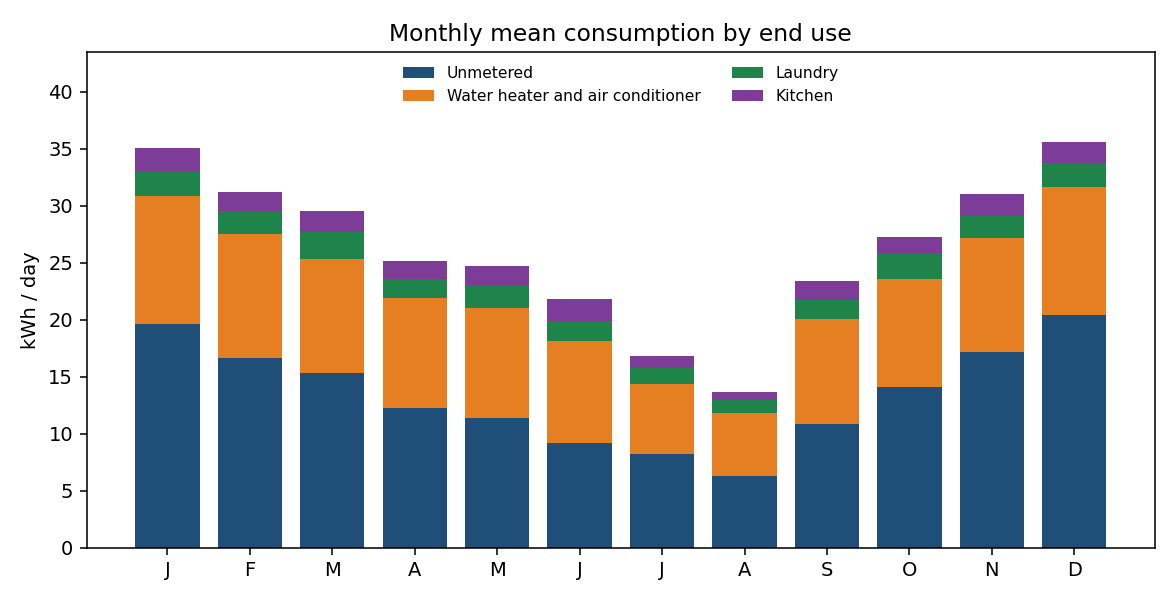
\includegraphics[width=0.92\textwidth]{figures/01d_enduse.png}
\caption{Monthly mean by end use. The unmetered remainder and the water-heater
circuit move with the season. Kitchen and laundry stay small in every month.}
\end{figure}

Just over half of a typical day, $13.41\kwh$ of $26.19$, is on none of the
three sub-meters. That remainder is lighting, electronics, and --- in this
house --- heating. Sub-meter 3, which the dataset labels as the water heater
and an air conditioner, is $9.30\kwh$ a day, 35\% of the total. Laundry is
$1.87$ and the kitchen is $1.61$.

The December-minus-August gap is $22.0\kwh$ a day if every August day is kept,
vacancies included. Of that gap, 65\% is unmetered and 26\% is sub-meter 3.
Kitchen and laundry together are about 10\%. Drop the vacancy blocks and
December still sits $17.3\kwh$ above August, of which $12.3\kwh$ is unmetered.
The annual cycle is heating and hot water.

Sub-meter 3 itself falls from $11.2\kwh$ a day in January to $6.2$ in July.
An air conditioner would rise in summer. In this house the circuit falls as
the weather warms, which is what an electric water heater does when the inlet
water is warmer. The air-conditioner half of the label does not show up in the
seasonal totals.

\subsection{The weekend effect is about 8 kWh in winter and about 2 kWh in summer}

\begin{center}
\small
\begin{tabular}{@{}lrr@{}}
\toprule
Contrast & kWh/day & 95\% interval \\
\midrule
Mon & -2.19 & [-2.93,\ -1.46] \\
Tue & -0.55 & [-1.35,\ +0.25] \\
Wed & -0.23 & [-1.07,\ +0.61] \\
Thu & -2.69 & [-3.48,\ -1.90] \\
Fri & -1.12 & [-1.88,\ -0.36] \\
Sat & +3.69 & [+2.69,\ +4.70] \\
Sun & +3.09 & [+2.03,\ +4.15] \\
\addlinespace
Winter weekend $-$ weekday & +7.99 & [+5.24,\ +10.73] \\
Spring weekend $-$ weekday & +5.24 & [+3.18,\ +7.31] \\
Summer weekend $-$ weekday & +2.14 & [+0.79,\ +3.48] \\
Autumn weekend $-$ weekday & +3.70 & [+1.83,\ +5.56] \\
\bottomrule
\end{tabular}

\end{center}

\noindent
The first seven rows are deviations from the seven-day mean, after month
indicators. Saturday is $+3.69\kwh$ and Sunday $+3.09$. Monday is $-2.19$ and
Thursday $-2.69$. Tuesday and Wednesday are compatible with the weekly mean.
The pooled weekend premium is $+4.75\kwh$ a day.

That pooled number is an average of two different seasons. In winter the
weekend premium is $+7.99\kwh$ a day, with interval $[+5.24,\ +10.73]$. In
summer it is $+2.14\kwh$, with interval $[+0.79,\ +3.48]$. Winter's interval
lies entirely above summer's. The additive day-of-week term in the Bayesian
model reports the average of the two. A winter Saturday sits well above it.

The circuits say why. In winter, Saturday averages $40.7\kwh$ and Monday
$30.5$. Of the $10.1\kwh$ gap, $4.4$ is unmetered, $2.1$ is laundry, $1.9$ is
the kitchen, and $1.7$ is the water heater. In summer the same
Saturday-minus-Monday gap is $2.2\kwh$, and the unmetered channel contributes
$0.3$ of it. Summer weekends are extra cooking and laundry. Winter weekends
are those, plus the heating, because someone is home.

Winter laundry has its own routine: about $2.9\kwh$ on Wednesday and
$3.0$--$3.3$ at the weekend, against about $1\kwh$ on Monday and Thursday.
That accounts for a large part of Thursday's winter deficit relative to
Wednesday. The data do not identify a calendar cause beyond that routine.

\begin{figure}[htbp]
\centering
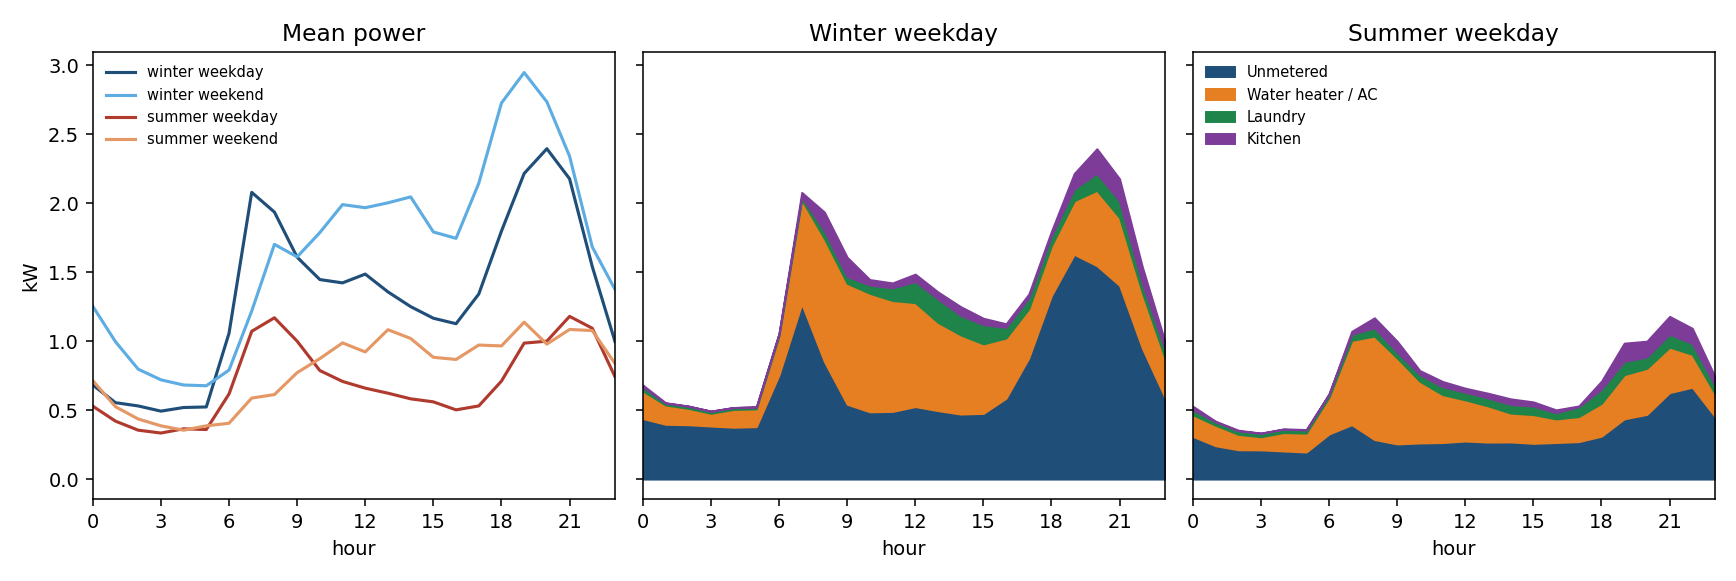
\includegraphics[width=\textwidth]{figures/01d_diurnal.png}
\caption{Left: mean power by hour in winter (December--February) and summer
(June--August). Centre and right: the weekday profiles split by end use. A
winter weekday integrates to $31.7\kwh$ and a summer weekday to $16.9\kwh$.}
\end{figure}

The hour of day is the same fact, finer. A winter weekday integrates to
$31.7\kwh$ and a winter weekend day to $39.7$; a summer weekday integrates to
$16.9$ and a summer weekend day to $18.9$. The differences, $8.0$ and
$2.0\kwh$, match the regression. Overnight, a winter weekday sits at
$0.52\,\mathrm{kW}$ and a summer weekday at $0.37\,\mathrm{kW}$. The evening
peak is $2.39\,\mathrm{kW}$ on a winter weekday and $1.18\,\mathrm{kW}$ on a
summer weekday.

At 07:00 on a winter weekday the load is $2.08\,\mathrm{kW}$, of which $1.27$
is unmetered and $0.75$ is the water heater. At 07:00 on a winter weekend it
is $1.22\,\mathrm{kW}$: the house wakes later. The summer spike at 07:00 is
$1.07\,\mathrm{kW}$, and $0.61$ of that is the water heater. Heating dominates
the winter peaks. The water heater dominates what is left of a summer morning.

Missing minutes are spread evenly across the clock, between 1.0\% and 1.4\% of
rows in every hour, so this shape is not an hour at which the meter drops out.
The 23 discarded days form eight short runs. The longest is 17--22 August 2010.

\subsection{Any trend is a few tenths of a kWh per year}

\begin{center}
\small
\begin{tabular}{@{}lrrr@{}}
\toprule
Sample & $n$ & Slope (kWh/year) & 95\% interval \\
\midrule
All retained days & 1417 & -0.358 & [-0.976,\ +0.260] \\
Drop 2006 & 1402 & -0.205 & [-0.799,\ +0.389] \\
Drop low-use blocks & 1360 & -0.427 & [-1.005,\ +0.151] \\
Complete years 2007-2009 & 1088 & -0.507 & [-1.382,\ +0.368] \\
\bottomrule
\end{tabular}

\end{center}

\noindent
The slope is the coefficient on $t/365$, with month and day-of-week indicators
in the same regression, so the annual cycle is saturated rather than left to
two harmonics. Every cut has a negative point estimate, between $-0.21$ and
$-0.51\kwh$ per year, and every interval covers zero. Dropping December 2006
moves the estimate from $-0.36$ to $-0.21$, because that fortnight is high and
it sits at the start of the series. The sign is negative either way. Four
years of one house cannot separate a drift of this size from no drift.

\subsection{On the kWh scale the memory is short, and both tails are heavy}

\begin{figure}[htbp]
\centering
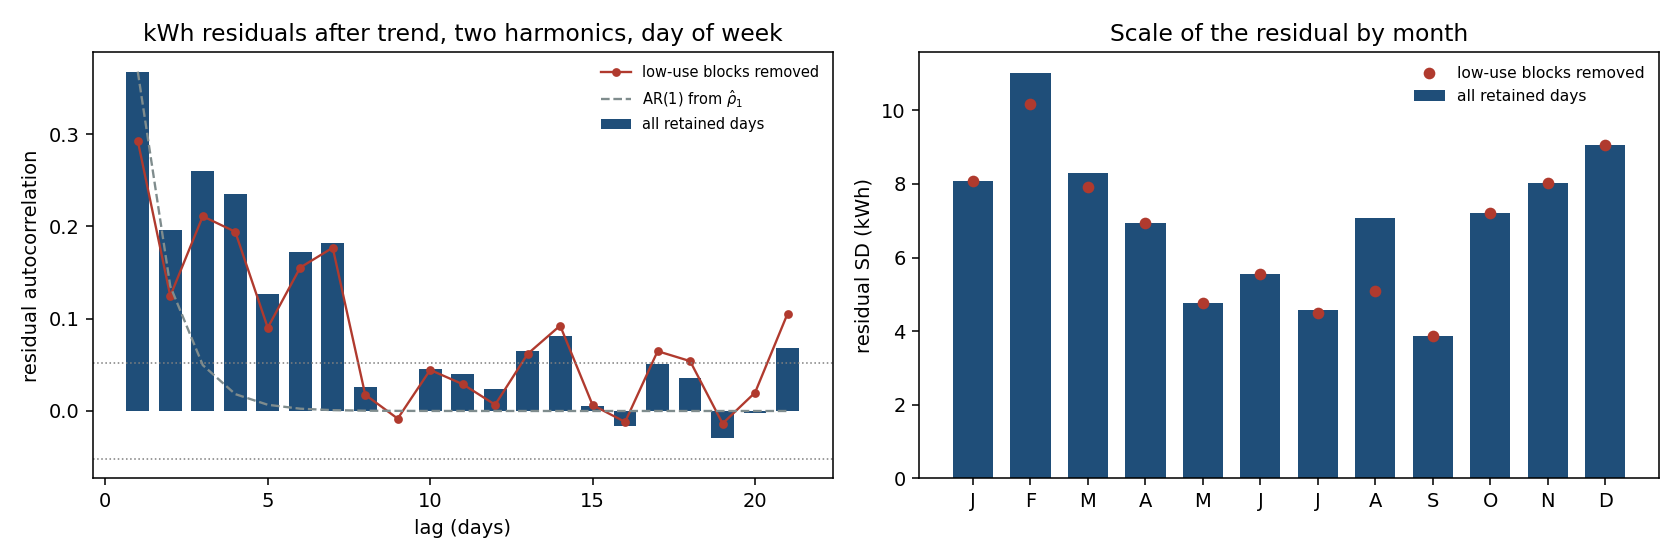
\includegraphics[width=\textwidth]{figures/01d_residual.png}
\caption{Residuals after a trend, two harmonics, and day of week, on the kWh
scale. Left: autocorrelation, with the low-use blocks removed in red, against
the geometric decay an AR(1) would produce. Right: residual standard deviation
by month. August drops once the vacancies are removed. February does not.}
\end{figure}

The earlier autocorrelation plot was on the log scale, where lag 1 is $0.58$
and the slow decay is largely the vacancy blocks. On the kWh scale, lag 1 is
$0.37$. An AR(1) with that coefficient makes a long-horizon band only about
7\% wider than a one-day-ahead band. That is the descriptive version of the
forecast result: knowing yesterday helps for a few days and then stops.

Removing the vacancy blocks lowers lag 1 to $0.29$. The rest is still not a
geometric decay. Lag 3 stays near $0.21$. Lag 7 stays near $0.18$ in the
autocorrelation, but its partial autocorrelation is about $0.05$, so little of
it is a weekly cycle left over after the day-of-week terms.

The heavy tail is real, and it is broader than the four long absences.
Residual kurtosis is about $5$, against $3$ for a Gaussian. The four blocks
are 4\% of days and 11\% of the residual sum of squares. The worst 5\% of days
hold 40\% of that sum of squares, split about evenly between winter spikes and
short low days. Only 11 of those 71 extreme days sit inside the long blocks.
The largest single residual is 23 December 2006, at $+39.8\kwh$. A $t$
innovation has both tails to absorb.

The spread is also seasonal. After the mean structure, winter residuals have
standard deviation $9.4\kwh$ and summer residuals $6.1$; without the blocks
the two numbers are $9.1$ and $5.1$. February stays near $10\kwh$. September
is $3.9\kwh$. A single innovation variance averages a volatile February and a
quiet September.

\section{What this changes in the model, and what it does not}

The deeper look supports the choices the holdout already made, and it names
three approximations those choices leave in place.

The kWh scale is the right one to model on. Logging turns the vacancy floor
into extreme left outliers and inflates the apparent memory. Two harmonics are
enough to carry the season; they are not enough to reproduce every wiggle, but
the missing piece is small in $R^2$. An AR(1) is a fair summary of the
short-run dependence. A heavy-tailed innovation is earned by the winter spikes
as well as by August.

Three things an additive model averages over, and which the exploratory
analysis can now state in kWh:

\begin{itemize}
\item The weekend premium is about $8\kwh$ a day in winter and about $2\kwh$
a day in summer.
\item August's raw mean mixes an occupied summer near $18\kwh$ with an empty
house near $5\kwh$. A day-of-year climatology trained through 2009 folds the
2008 vacancy into mid-August, and the test year is vacant over some of the
same dates.
\item Winter days are more variable than summer days even after the vacancies
are removed, and February in particular still looks like weather rather than
occupancy. There is no temperature series in the model.
\end{itemize}

The numbers in the main report's posterior summaries remain the ones to quote
for the scientific questions. This note is what those summaries are describing.

\end{document}
